\documentclass[a4paper, twocolumn]{article}
\usepackage[utf8]{inputenc}
\usepackage[english]{babel}
\usepackage{graphicx}
\usepackage{wrapfig}
\usepackage{lipsum}
\usepackage{multicol}
\usepackage{hyperref}
\usepackage{enumitem}
\usepackage{float}
\usepackage{tikz}
\usetikzlibrary{shapes, arrows.meta, positioning}
\usepackage[margin=1in]{geometry}
\setlength{\parskip}{0.3em}
\setlength{\columnsep}{20pt}
\date{}
\raggedbottom
\raggedcolumns

\title{\textbf{Machine Learning Approaches to Classify Topics in Forums}}
\author{Sitong Liu \\ stliu@unc.edu}

\begin{document}

\maketitle

\section{Introduction}

Against the background of today's rapid Internet development, online forums have become an important platform for university students to discuss course content and communicate about campus life. Triple Uni is a typical example, a forum shared by students from the University of Hong Kong (HKU), the Chinese University of Hong Kong  (CUHK) and the Hong Kong University of Science and Technology (HKUST). As the forum expands and the number of posts increases, content retrieval is challenged by the massive amount of information.

One solution is to encourage users to actively tag posts with topics so that other users can more accurately find the information they need. However, the reality is that not all users are happy to actively tag posts. Many users, when asked by the system, just randomly select a topic from the list of topics to pass the validation, which reduces the differentiation and usefulness of topic tags.

In this study, machine learning approaches are used to automatically classify posts with the aim of improving classification accuracy and optimizing user experience. Specific methods include training three classifiers, random forest classifier, softmax classifier and neural network classifier, and comparing their performance to determine the most suitable machine learning model for this forum.

\section{Dataset and Data Cleaning}

\subsection{Dataset Description}

The dataset collected for this study is from the Triple Uni and includes half a million posts numbered 1 to 500000 and user-selected topics on the platform. This study applies the text-embedding-ada-002 model provided by OpenAI to embed the post text and generates a 1536-dimensional representation vector. To follow the privacy rules of the platform, we desensitize the raw text in the dataset and keep only the corresponding text-embedding vectors. The structure of the dataset is as follows:

\begin{table}[H]
\centering
\footnotesize
\begin{tabular}{|c|c|c|}
\hline
\textbf{Field Name} & \textbf{Type} & \textbf{Description} \\ \hline
uni\_post\_id & int64 & Post id of the forum\\ \hline
post\_topic & string & Topic of the post (in Chinese) \\ \hline
embedding & float[1536] & Embedding of the post content \\ \hline
\end{tabular}
\caption{Dataset Structure}
\end{table}

\subsection{Data Cleaning}

In order to cope with the change in the platform's topic categorization, we decide to select the target topics as Trading, Academics, Emotions, Job Hunting and Random Thoughts. In this study, we re-classify the topics with similar meanings to these target topics into the designated topics and exclude all other topics. Given that the original topics are in Chinese, we also convert these topics into English representations. The specific topics are classified as follows: 

\begin{table}[H]
\centering
\begin{tabular}{|c|c|c|}
\hline
\textbf{Topic in English} & \textbf{Count} \\ \hline
Trading & 15963 \\ \hline
Academics & 88468 \\ \hline
Emotions & 44848\\ \hline
Job Hunting & 11105 \\ \hline
Random Thoughts & 141586 \\ \hline
\end{tabular}
\caption{Topics List}
\end{table}

\subsection{Data Splitting}

The dataset is divided into two parts: 80\% for the training set and 20\% for the test set. The aim of this move is to verify that our model is able to show excellent performance on unseen data, rather than just overfitting on the training data. 

\subsection{Data Accessibility}

The dataset for this study is publicly available at \href{https://drive.google.com/drive/u/1/folders/1VVpugGyS-9-mhkvHh4wTX-feFAt3hEVP}{https://drive.google.com/drive/u/1/folders/1VVpugGyS-9-mhkvHh4wTX-feFAt3hEVP}.

\section{A Closer Look at the Data}

In order to visualize the relationship between embedding and topic categories, this study adopts the t-SNE method to reduce embedding from high dimensionality to 2 dimensionality while preserving the relative position information. By using different colors to identify each topic, we achieve a visual presentation of the data.

\begin{figure}[ht]
\begin{center}
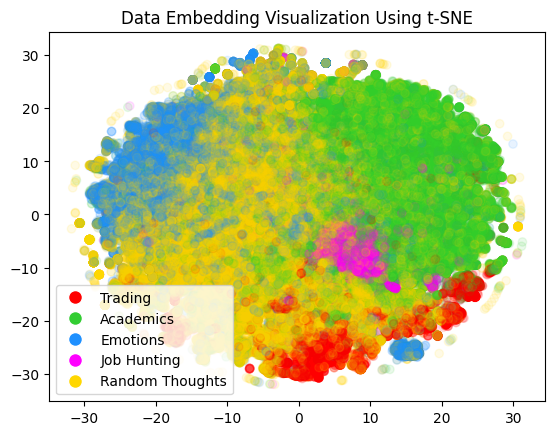
\includegraphics[width=1\linewidth]{Figure1.png}
\end{center}
\end{figure}

We observe that posts on the same topics tend to cluster together in the graph, which validates the feasibility of classifying posts using machine learning's embedding technique. In particular, posts on the topics of Job Hunting and Academics form tight clusters in the graph, showing a high degree of correlation between posts of these topics, signaling that these topics may perform better in the classification task. On the contrary, posts on the topic of Random Thought are more scattered in the graph, which may be due to the fact that Random Thought  covers a wider range of content, and other posts that are not easy to categorize may be classified as this topic, making it more difficult to categorize them.

Since topics are specified by users, their accuracy cannot be guaranteed. As a result, many outliers appear on the graph, and these may indicate errors in the topic labeling of posts. How to minimize the impact of these mislabeled data is a major challenge for us. In addition, the uneven number of posts across topics poses an additional difficulty to the classification task.

\section{Models and Training}

In order to select the best model, this study analyzes the data using random forest, softmax regression and neural network respectively and compares their accuracy.

\subsection{Random Forest}

According to Breiman (2001), random forest models are very effective in dealing with high dimensional data, can effectively prevent overfitting and are more resistant to interference with mislabeled training data.

We train a random forests model with 100 estimators using the training set and test the model on the test set. On the test set, the model achieved an accuracy of 70.9027\%.

\begin{figure}[ht]
\begin{center}
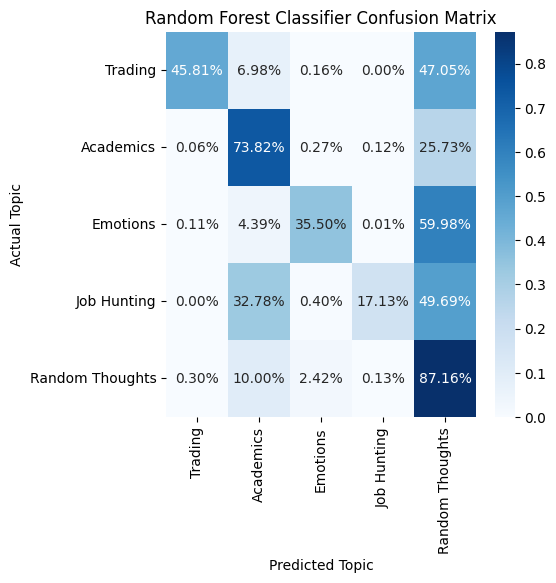
\includegraphics[width=1\linewidth]{Figure2.png}
\end{center}
\end{figure}

Although the accuracy is not low, we find that random forest model does not handle the unbalanced training data well. Nearly half of the training data is in the Random Thought category, which leads to a tendency for the model to predict most inputs as Random Thought topics, and thus random forest does not perform well on this dataset.

\subsection{Softmax Regression}

Bishop (2006) describes softmax regression as a generalization of logistic regression that is applicable to multi-class classification problems, where it calculates the probabilities of each class over all possible classes.

In order to solve the problem of unbalanced training data, we optimize the cross-entropy loss function and introduce a weighted loss function based on the proportion of categories. This function takes into account the proportions of different categories and imposes higher penalties for classification errors in niche categories, thus improving the model's classification of all categories.

We set the batch size to 256, the learning rate to 0.001 and set the epochs to 50 and use these parameters to train the softmax model. The model achieves 74.2921\% accuracy on the test set.

\begin{figure}[ht]
\begin{center}
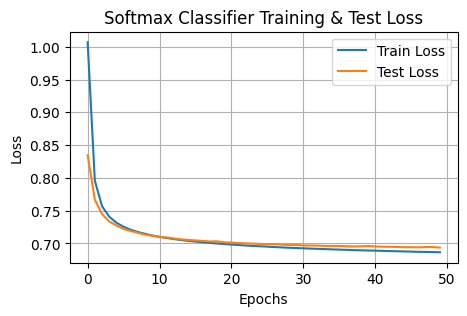
\includegraphics[width=1\linewidth]{Figure3.png}
\end{center}
\end{figure}

\begin{figure}[ht]
\begin{center}
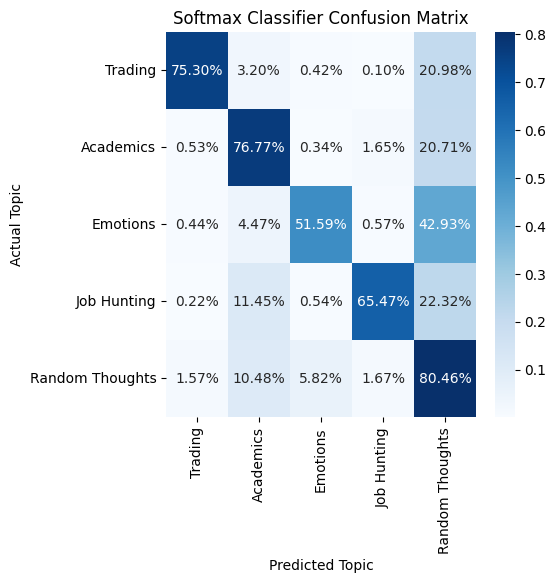
\includegraphics[width=1\linewidth]{Figure4.png}
\end{center}
\end{figure}

The softmax model achieves higher accuracy compared to random forest and effectively mitigates the unbalanced training data problem. Moreover, due to the simpler model structure, softmax is significantly faster than random forest in both training and inference. All these indicate that softmax is the superior choice in this problem.

\subsection{Neural Network}

As highlighted by LeCun, Bengio, and Hinton (2015), neural networks have been pivotal in advancing classification tasks across various domains, harnessing their ability to learn complex patterns through deep architectures.

We use the most basic neural network model, which consists of three fully connected layers, each followed by a batch normalization and ReLU activation function. To prevent overfitting, a Dropout layer with a dropout rate of 0.5 is added after the first and second fully connected layers. The structure of the model starts with an input layer, first a fully connected layer that maps the input dimensions to 128, then through a 32-dimensional and a 16-dimensional fully connected layer, and finally through an softmax layer that produces predictions.

\begin{figure}[h!]
\begin{center}
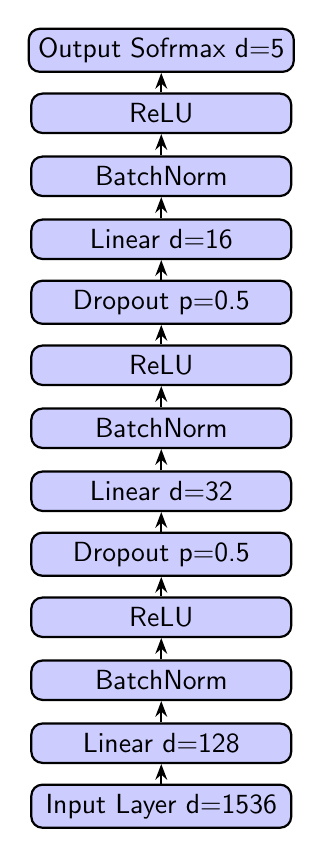
\begin{tikzpicture}[
    node distance=0.8cm,
    line width=1pt,
    >={Stealth[length=2mm]},
    every node/.style={font=\sffamily, align=center},
    layer/.style={draw, thick, rounded corners, minimum width=3.3cm, minimum height=0.5cm, fill=blue!20},
    arrow/.style={->, thick}
]
\node[layer] (input) {Input Layer d=1536};
\node[layer, above of=input] (linear1) {Linear d=128};
\node[layer, above of=linear1] (batchnorm1) {BatchNorm};
\node[layer, above of=batchnorm1] (relu1) {ReLU};
\node[layer, above of=relu1] (dropout1) {Dropout p=0.5};
\node[layer, above of=dropout1] (linear2) {Linear d=32};
\node[layer, above of=linear2] (batchnorm2) {BatchNorm};
\node[layer, above of=batchnorm2] (relu2) {ReLU};
\node[layer, above of=relu2] (dropout2) {Dropout p=0.5};
\node[layer, above of=dropout2] (linear3) {Linear d=16};
\node[layer, above of=linear3] (batchnorm3) {BatchNorm};
\node[layer, above of=batchnorm3] (relu3) {ReLU};
\node[layer, above of=relu3] (output) {Output Sofrmax d=5};
\draw[arrow] (input) -- (linear1);
\draw[arrow] (linear1) -- (batchnorm1);
\draw[arrow] (batchnorm1) -- (relu1);
\draw[arrow] (relu1) -- (dropout1);
\draw[arrow] (dropout1) -- (linear2);
\draw[arrow] (linear2) -- (batchnorm2);
\draw[arrow] (batchnorm2) -- (relu2);
\draw[arrow] (relu2) -- (dropout2);
\draw[arrow] (dropout2) -- (linear3);
\draw[arrow] (linear3) -- (batchnorm3);
\draw[arrow] (batchnorm3) -- (relu3);
\draw[arrow] (relu3) -- (output);
\end{tikzpicture}
\end{center}
\end{figure}

We train the neural network model with a batch size of 256, a learning rate of 0.001, and with 20 training cycles. With these settings, the model achieves 75.7923\% accuracy on the test set.

\begin{figure}[ht]
\begin{center}
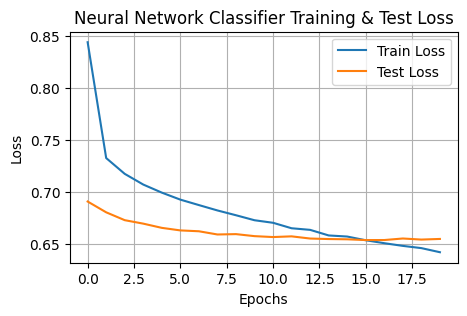
\includegraphics[width=1\linewidth]{Figure5.png}
\end{center}
\end{figure}

\begin{figure}[ht]
\begin{center}
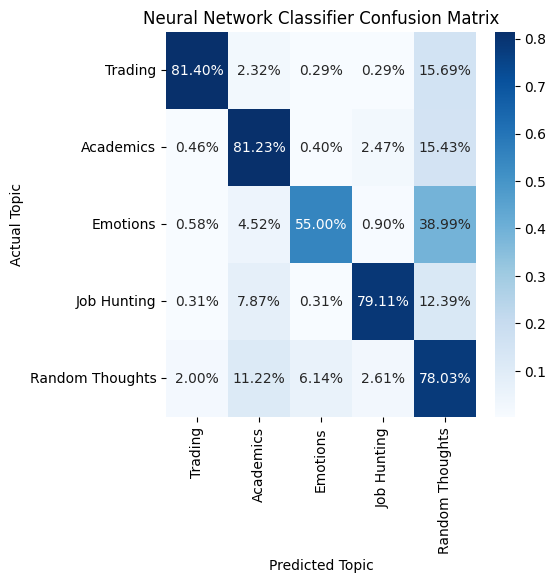
\includegraphics[width=1\linewidth]{Figure6.png}
\end{center}
\end{figure}

There is a further improvement in the model accuracy of the neural network, while the unbalanced training data problem is further mitigated. This suggests that increasing the depth of the network helps to improve the model's ability to generalize. However, the model is still more difficult to distinguish between Random Thought and Emotions, which may be due to the fact that the content of the posts under these two topics is relatively similar without clear boundaries. In addition, the training and inference speed of the neural network model is significantly slower than that of the softmax model, and in practical applications, we need to consider the cost and effect together to choose the most suitable model.

\section{Summary}

\subsection{Models Comparison}

\begin{table}[H]
\centering
\begin{tabular}{|c|c|c|}
\hline
\textbf{Model} & \textbf{Test Accuracy} \\ \hline
Random Forest&70.9027\%\\ \hline
Softmax Regression&74.2921\%\\ \hline
Neural Network&75.7923\%\\ \hline
\end{tabular}
\caption{Models Comparison}
\end{table}

\subsection{Conclusion}

In this study, we test the performance of multiple machine learning techniques on a topic classification task. The results show that the model containing a softmax layer outperforms the random forest model, while the neural network model further outperforms the softmax regression model in terms of accuracy. Nevertheless, the overhead of neural networks is significantly higher than that of the softmax regression model, both in terms of training and inference, making the latter a more cost-effective option.

Further improvement of model accuracy is challenged by the limitations of data labeling. One potential solution is to manually calibrate the data labels of the test set, which would provide more reliable metrics for evaluating model effectiveness. However, due to time and resource constraints, this method could not be implemented in this study, which would be an important direction for future research.

\subsection{Live Demo}

We develop an live demo application using Streamlit which allows the user to enter a text and shows the classification results of different models. You can experience the performance of these models by visiting \href{https://tree-hole-judge.tripleuni.com/}{https://tree-hole-judge.tripleuni.com/}.

\subsection{Code Accessibility}

The code for our data cleaning, model training, as well as the live demo, are all open source and available at the following GitHub link \href{https://github.com/lststar/Triple-Uni-Topic-Classifier}{https://github.com/lststar/Triple-Uni-Topic-Classifier}.

\newpage

\begin{thebibliography}{3}

\bibitem{Breiman2001} 
Breiman, L. (2001). Random Forests. 
\textit{Machine Learning}, 45(1), 5-32.
\url{https://doi.org/10.1023/A:1010933404324}.

\bibitem{Bishop2006} 
Bishop, C. M. (2006).
\textit{Pattern Recognition and Machine Learning}.
\url{https://doi.org/10.1007/978-0-387-45528-0}.

\bibitem{LeCun2015} 
LeCun, Y., Bengio, Y., \& Hinton, G. (2015). Deep learning.
\textit{Nature}, 521(7553), 436-444.
\url{https://doi.org/10.1038/nature14539}.

\end{thebibliography}

\end{document}